% The Clever Algorithms Project: http://www.CleverAlgorithms.com
% (c) Copyright 2011 Jason Brownlee. Some Rights Reserved. 
% This work is licensed under a Creative Commons Attribution-Noncommercial-Share Alike 2.5 Australia License.

% Name
% The algorithm name defines the canonical name used to refer to the technique, in addition to common aliases, abbreviations, and acronyms. The name is used in terms of the heading and sub-headings of an algorithm description.
\section{Ordinary Least Squares Regression} 
\label{sec:ordinary}
\index{Ordinary Least Squares Regression}
\index{Ordinary Linear Regression}
\index{Linear Least Squares}

% other names
% What is the canonical name and common aliases for a technique?
% What are the common abbreviations and acronyms for a technique?
\emph{Ordinary Least Squares Regression, Ordinary Linear Regression, OLS, OLSR, Linear Least Squares}

% Taxonomy: Lineage and locality
% The algorithm taxonomy defines where a techniques fits into the field, both the specific subfields of Computational Intelligence and Biologically Inspired Computation as well as the broader field of Artificial Intelligence. The taxonomy also provides a context for determining the relation- ships between algorithms. The taxonomy may be described in terms of a series of relationship statements or pictorially as a venn diagram or a graph with hierarchical structure.
\subsection{Taxonomy}
% To what fields of study does a technique belong?
Ordinary Least Squares is a method for estimating the parameters for a linear regression model.
% What are the closely related approaches to a technique?
It is related to other least squares methods for estimating the parameters of linear models such as Weighted Least Squares and Partial Least Squares.

% Strategy: Problem solving plan
% The strategy is an abstract description of the computational model. The strategy describes the information processing actions a technique shall take in order to achieve an objective. The strategy provides a logical separation between a computational realization (procedure) and a analogous system (metaphor). A given problem solving strategy may be realized as one of a number specific algorithms or problem solving systems. The strategy description is textual using information processing and algorithmic terminology.
\subsection{Strategy}
% What is the information processing objective of a technique?
The information processing objective of the Ordinary Least Squares Method is define a line a best fit.
% What is a techniques plan of action?
The line is defined by an equation that minimizes the Sum of the Squared Residuals (SSR) with an intercept and a regression coefficient.

% Heuristics: Usage guidelines
% The heuristics element describe the commonsense, best practice, and demonstrated rules for applying and configuring a parameterized algorithm. The heuristics relate to the technical details of the techniques procedure and data structures for general classes of application (neither specific implementations not specific problem instances). The heuristics are described textually, such as a series of guidelines in a bullet-point structure.
\subsection{Heuristics}
% What are the suggested configurations for a technique?
% What are the guidelines for the application of a technique to a problem instance?

\begin{itemize}
	\item An OLS model is asymptotically consistent when 1) the errors are unbiased (zero mean) and 2) the coefficients (regressors) are linearly independent.
	\item The Gauss-Markov theorem indicates that a linear regression model where 1) all errors have the same variance (hoemoscedasticity), and 2) all errors are drawn from uncorrelated distributions (nonautocorrelation) then the coefficients given by OLS result in the Best Linear Unbiased Estimator (BLUE).
	\item Under the Gauss-Markov conditions, if the errors are further 1) independent and identically distributed (iid), and 2) drawn from a normal distributions then the models estimates may be taken as maximum likelihood estimates.
	\item the model assumes attributes are drawn from a normal distribution and a straight line can be drawn through the mean (under the normal and iid assumptions).
	\item The dependent variable must be continuous, but the independent variables may be continuous or categorical.
	\item Relative to modern methods the prediction accuracy is poor and interpretation of the model can be difficult.
	\item An $R^2$ statistic can be used to indicate the ``goodness of fit'' of a resulting regression line. It represents the proportion of the variance of the dependent variable that can be explained by the independent variables. An $R^2=1$ is a perfect fit, and an $R^2=0$ when the coefficients cannot explain any observations.
	\item The magnitude of a coefficient indicates the relative importance of its independent variable to the model.
\end{itemize}


% sample script in R
\subsection{Code Listing}
% listing
Listing~\ref{stats_ordinary_least_squares} provides a code listing Ordinary Least Squares method in R. Figure~\ref{plot:ordinary_least_squares_regression_result} provides a plot of the training dataset with the line of best fit highlighted.

% algorithm and package
The example uses the \texttt{lm()} function in the \texttt{stats} core package which is responsible for fitting linear least squares models.
% problem
The test problem is a two-dimensional dataset of 100 samples, where the \texttt{x}-values are drawn from a uniformly random distribution $x \in [0,10]$ and \texttt{y} values are the \texttt{x} value plus a value drawn from a normally random distribution with a mean of 0 and a standard deviation of 1.

% classification example?

\lstinputlisting[firstline=7,language=r,caption={Example of Ordinary Least Squares in R using the \texttt{lm()} function in the \texttt{stats} core package.}, label=stats_ordinary_least_squares]{../src/algorithms/regression/stats_ordinary_least_squares.R}

\begin{figure}[htp]
\centering
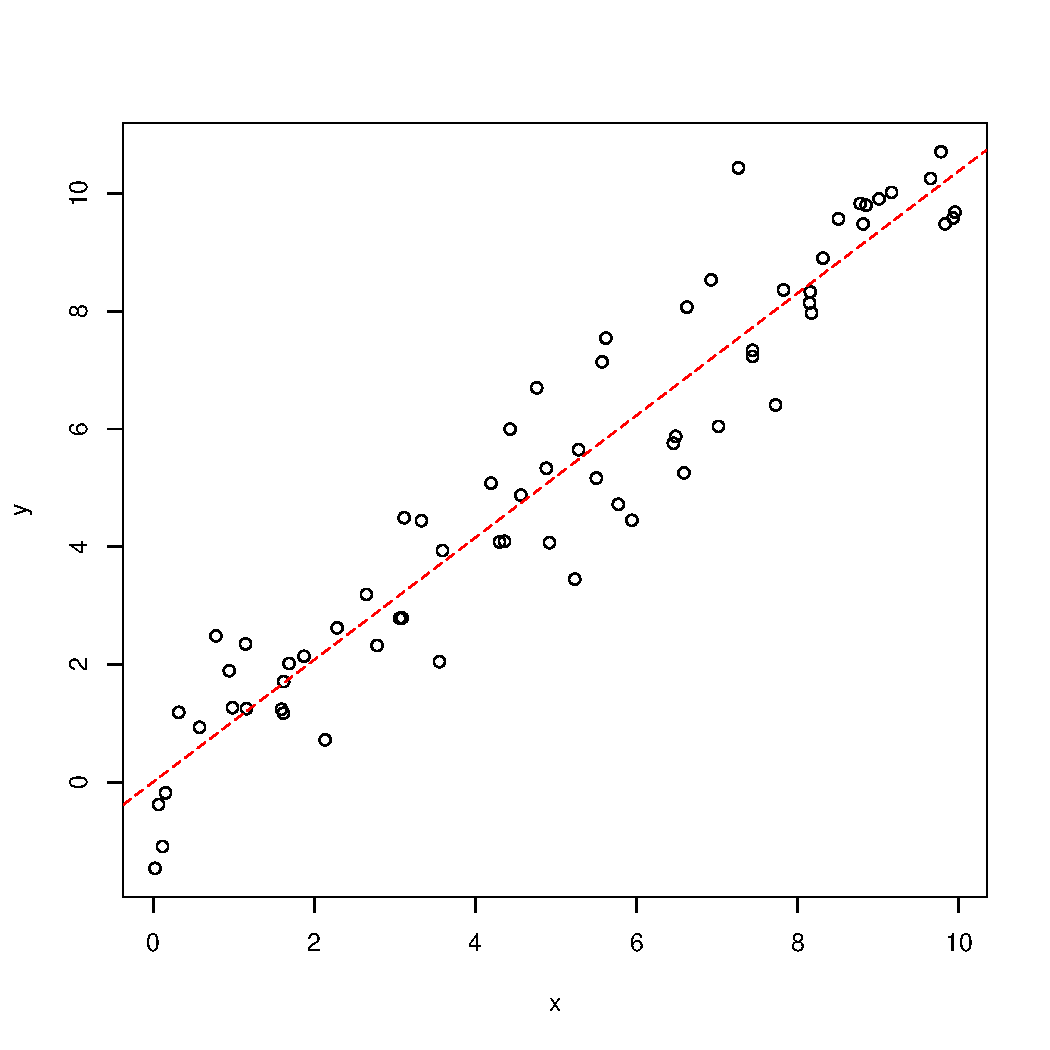
\includegraphics[scale=0.45]{a_regression/ordinary_least_squares_regression_result.pdf}
\caption{Plot 2D training dataset with the line of best fit.}
\label{plot:ordinary_least_squares_regression_result}
\end{figure}

% other packages ?


% References: Deeper understanding
% The references element description includes a listing of both primary sources of information about the technique as well as useful introductory sources for novices to gain a deeper understanding of the theory and application of the technique. The description consists of hand-selected reference material including books, peer reviewed conference papers, journal articles, and potentially websites. A bullet-pointed structure is suggested.
\subsection{References}
% What are the primary sources for a technique?
% What are the suggested reference sources for learning more about a technique?

% primary sources
\subsubsection{Primary Sources}
% least squares
The method for Least Squares may be traced back to Gauss who claims to have devised the method in and later published it in 1809 \cite{Gauss1809, Gauss1823} (German). Legendre independently developed and published the Least Squares method in 1805 \cite{Legendre1805} (Appendix, French).
% ordinary least squares specifically

% more info
\subsubsection{More Information}
% text books
Least Squares regression is covered in any good text of statistics, data analysis or econometrics. Some popular introductory texts to least squares regression include Montgomery et~al.\ \cite{Montgomery2001} (Chapter 2), and Tamhane and Dunlop \cite{Tamhane2000} (Chapter 10).
% in R
Faraway provides a free book that includes a practical introduction into Least Squares Regression with examples in R \cite{Faraway2002} (updated version published \cite{Faraway2004}).


% END
